\documentclass[a4paper,11pt]{article}

\usepackage{pgfplots}
\usepackage{tikz}
\usepackage{subfigure}
\usepackage[top=3cm,bottom=3cm,left=2.5cm,right=2.5cm]{geometry}

\begin{document}

\begin{figure}[t!]
	\centering
	\subfigure[High learning rate.]{
    		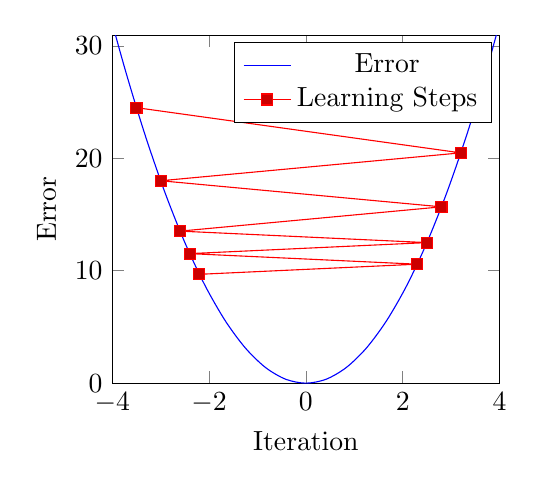
\begin{tikzpicture}
			\begin{axis}[height=6cm,width=6.5cm,ylabel=Error,xlabel=Iteration,xmin=-4,xmax=4,ymin=0]
				\addplot[blue,smooth] {2*x^2};
				\addlegendentry{Error}
				\addplot+[red] coordinates{(-3.5,24.5)(3.2,20.48)(-3,18)(2.8,15.68)(-2.6,13.52)(2.5,12.5)(-2.4,11.52)(2.3,10.58)(-2.2,9.68)};
				\addlegendentry{Learning Steps}
			\end{axis}
		\end{tikzpicture}
		\label{subfig:momentum-high}
	}
	\subfigure[Low learning rate.]{
		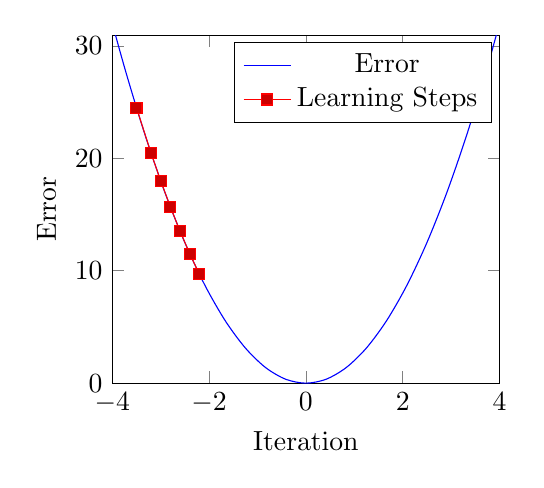
\begin{tikzpicture}
			\begin{axis}[height=6cm,width=6.5cm,ylabel=Error,xlabel=Iteration,xmin=-4,xmax=4,ymin=0]
				\addplot[blue,smooth] {2*x^2};
				\addlegendentry{Error}
				\addplot+[red] coordinates{(-3.5,24.5)(-3.2,20.48)(-3,18)(-2.8,15.68)(-2.6,13.52)(-2.4,11.52)(-2.2,9.68)};
				\addlegendentry{Learning Steps}
			\end{axis}
		\end{tikzpicture}
		\label{subfig:momentum-low}
	}
    	\caption[The learning rate and its influence on the rate of convergence.]{When using a large learning rate the weight updates in each iteration tend to overstep the minimum. This causes oscillation around the minimum. This observation is illustrated by figure \ref{subfig:momentum-high}. Choosing the learning rate too low will result in a slow convergence to the minimum as shown in figure \ref{subfig:momentum-low}. Both scenarios are visualized using a quadratic function we seek to minimize.}
    	\label{fig:momentum}
\end{figure}

\end{document}